\documentclass[12pt,letterpaper]{article}\usepackage[]{graphicx}\usepackage[]{color}
%% maxwidth is the original width if it is less than linewidth
%% otherwise use linewidth (to make sure the graphics do not exceed the margin)
\makeatletter
\def\maxwidth{ %
  \ifdim\Gin@nat@width>\linewidth
    \linewidth
  \else
    \Gin@nat@width
  \fi
}
\makeatother

\definecolor{fgcolor}{rgb}{0.345, 0.345, 0.345}
\newcommand{\hlnum}[1]{\textcolor[rgb]{0.686,0.059,0.569}{#1}}%
\newcommand{\hlstr}[1]{\textcolor[rgb]{0.192,0.494,0.8}{#1}}%
\newcommand{\hlcom}[1]{\textcolor[rgb]{0.678,0.584,0.686}{\textit{#1}}}%
\newcommand{\hlopt}[1]{\textcolor[rgb]{0,0,0}{#1}}%
\newcommand{\hlstd}[1]{\textcolor[rgb]{0.345,0.345,0.345}{#1}}%
\newcommand{\hlkwa}[1]{\textcolor[rgb]{0.161,0.373,0.58}{\textbf{#1}}}%
\newcommand{\hlkwb}[1]{\textcolor[rgb]{0.69,0.353,0.396}{#1}}%
\newcommand{\hlkwc}[1]{\textcolor[rgb]{0.333,0.667,0.333}{#1}}%
\newcommand{\hlkwd}[1]{\textcolor[rgb]{0.737,0.353,0.396}{\textbf{#1}}}%

\usepackage{framed}
\makeatletter
\newenvironment{kframe}{%
 \def\at@end@of@kframe{}%
 \ifinner\ifhmode%
  \def\at@end@of@kframe{\end{minipage}}%
  \begin{minipage}{\columnwidth}%
 \fi\fi%
 \def\FrameCommand##1{\hskip\@totalleftmargin \hskip-\fboxsep
 \colorbox{shadecolor}{##1}\hskip-\fboxsep
     % There is no \\@totalrightmargin, so:
     \hskip-\linewidth \hskip-\@totalleftmargin \hskip\columnwidth}%
 \MakeFramed {\advance\hsize-\width
   \@totalleftmargin\z@ \linewidth\hsize
   \@setminipage}}%
 {\par\unskip\endMakeFramed%
 \at@end@of@kframe}
\makeatother

\definecolor{shadecolor}{rgb}{.97, .97, .97}
\definecolor{messagecolor}{rgb}{0, 0, 0}
\definecolor{warningcolor}{rgb}{1, 0, 1}
\definecolor{errorcolor}{rgb}{1, 0, 0}
\newenvironment{knitrout}{}{} % an empty environment to be redefined in TeX

\usepackage{alltt}
\usepackage[left=2cm,right=2cm,top=2cm,bottom=2cm]{geometry}
\usepackage[ansinew]{inputenc}
\usepackage[spanish]{babel}
\usepackage{amsmath}
\usepackage{amsfonts}
\usepackage{amssymb}
\usepackage{dsfont}
\usepackage{multicol} 
\usepackage{subfigure}
\usepackage{graphicx}
\usepackage{float} 
\usepackage{verbatim} 
\usepackage[left=2cm,right=2cm,top=2cm,bottom=2cm]{geometry}
\usepackage{fancyhdr}
\pagestyle{fancy} 
\fancyhead[LO]{\leftmark}
\usepackage{caption}
\newtheorem{definicion}{Definci\'on}
\IfFileExists{upquote.sty}{\usepackage{upquote}}{}
\begin{document}

\begin{titlepage}
\setlength{\unitlength}{1 cm} %Especificar unidad de trabajo

\begin{center}
\textbf{{\large UNIVERSIDAD DE EL SALVADOR}\\ [0.50 cm]
{\large FACULTAD MULTIDISCIPLINARIA DE OCCIDENTE}\\ [0.50 cm]
{\large DEPARTAMENTO DE MATEM\'ATICA}}\\ [0.50 cm]

\begin{picture}(18,4)
 \put(7,0){
\includegraphics[width=4cm]{minerva.jpg}}
\end{picture}
\\[0.25 cm]

\textbf{{\large Licenciatura en Estad\'istica}\\ [1.25cm]
{\large Control Estad\'istico del Paquete R }\\ [2 cm]
%\setlength{\unitlength}{1 cm}
{\large  \textbf{''UNIDAD TRES"}}\\ [3 cm]
{\large Alumna:}\\
{\large Erika Beatr\'iz Guill\'en Pineda}\\ [2cm]
{\large Fecha de elaboraci\'on}\\
Santa Ana - \today }
\end{center}
\end{titlepage}

\newtheorem{teorema}{Teorema}
\newtheorem{prop}{Proposici\'on}[section]

\lhead{Pr?\'actica 15}

\lfoot{LICENCIATURA EN ESTAD\'ISTICA}
\cfoot{UESOCC}
\rfoot{\thepage}
%\pagestyle{fancy} 

\setcounter{page}{1}
\newpage


\section {DISTRIBUCIONES CONTINUAS.} 

\begin{description}
  \item \textbf{a) Distribuci\'on uniforme.}
\end{description}

\begin{itemize}
  \item \textbf{Par\'ametros.}
  \begin{center}
\item x = valor cualquiera
\item p = probabilidad
\item n = tama?o de la muestra 
\item min = valor m\'inimo
\item max = valor m\'aximo
\end{center}

\item \textbf{Sintaxis de la funci\'on utilizada en R}
\begin{enumerate}
  \item punif(x, min, max, lower.tail = TRUE, log.p = FALSE)
  \item qunif(p, min, max, lower.tail = TRUE, log.p = FALSE) 
  \item runif(n, min, max) 
\end{enumerate}
\end{itemize}

\begin{description}
  \item \textbf{b) Distribuci\'on Normal.}
\end{description}

\begin{itemize}
  \item \textbf{Par\'ametros.}
  \begin{center}
\item x = valor cualquiera
\item p = probabilidad
\item mean = media
\item sd = desviaci\'on t\'ipica
\item n = tama\~no de la muestra
\end{center}
\item \textbf{Sintaxis de la funci\'on utilizada en R}
\begin{enumerate}
  \item pnorm(x, mean, sd, lower.tail = TRUE, log.p = FALSE) 
  \item qnorm(p, mean, sd, lower.tail = TRUE, log.p = FALSE) 
  \item rnorm(n, mean, sd)  
\end{enumerate}
\end{itemize}

\begin{description}
  \item \textbf{c) Distribuci\'on T-Student.}
\end{description}
\begin{itemize}
  \item \textbf{Par\'ametros.}
  \begin{center}
\item x = valor cualquiera
\item p = probabilidad
\item df = grados de libertad  
\end{center}
\item \textbf{Sintaxis de la funci\'on utilizada en R}
\begin{enumerate}
  \item pt(x, df, lower.tail = TRUE, log.p = FALSE)
  \item pt(x, df, lower.tail = TRUE, log.p = FALSE) 
  \item rt(n, df)   
\end{enumerate}
\end{itemize}

\begin{description}
  \item \textbf{d) Distribui\'on Chi-cuadrado.}
\end{description}
\begin{itemize}
  \item \textbf{Par\'ametros.}
  \begin{center}
\item x = valor cualquiera
\item df = grados de libertad
\item p = probabilidad 
\end{center}
\item \textbf{Sintaxis de la funci\'on utilizada en R}
\begin{enumerate}
  \item pchisq(x, df, lower.tail = TRUE, log.p = FALSE)
  \item qchisq(p, df, lower.tail = TRUE, log.p = FALSE)
  \item rchisq(n, df,)    
\end{enumerate}
\end{itemize}

\begin{description}
  \item \textbf{d) Distribuci\'on F de Snedecor.}
\end{description}
\begin{itemize}
  \item \textbf{Par?metros.}
  \begin{center}
\item x,q = vector cuantiles
\item df1 = grados de libertad en el numerador
\item df2 = grados de libertad en el denominador 
\item p = vector probabilidad
\end{center}
\item \textbf{Sintaxis de la funci\'on utilizada en R}
\begin{enumerate}
  \item pf(q, df1, df2, ncp, lower.tail = TRUE, log.p = FALSE)
  \item qf(p, df1, df2, ncp, lower.tail=TRUE, log.p = FALSE) 
  \item rf(n, df1, df2, ncp) 
\end{enumerate}
\end{itemize}

\begin{description}
  \item \textbf{d) Distribuci\'on Exponencial.}
\end{description}
\begin{itemize}
  \item \textbf{Par\'ametros.}
  \begin{center}
\item x,q = vector cuantiles
\item rate = raz?n = 1/E[X]
\item p = vector probabilidad 
\item lower.tail = T 
\end{center}
\item \textbf{Sintaxis de la funci\'on utilizada en R}
\begin{enumerate}
  \item pexp(q, rate = 1, lower.tail = TRUE, log.p = FALSE)
  \item qexp(p, rate = 1, lower.tail = TRUE, log.p = FALSE)
  \item rexp(n, rate = 1)  
\end{enumerate}
\end{itemize}


\section{C\'ALCULO DE PROBABILIDADES.}

\begin{itemize}
  \item \textbf{Ejemplo 1:}
\end{itemize}

Una persona informal hace esperar a su pareja aleatoriamente entre 0 y 90 minutos. Harto de esta situaci\'on, la persona que sufre la espera se plantea un ultim\'atum; s\'i al d\'ia siguiente su pareja tarda menos de 15 minutos mantiene la relaci\'on, s\'i la espera est\'e entre 15 y 55 minutos, decide en la siguiente cita con los mismos criterios, mientras que si tarda m\'as de 55 minutos la relaci\'on termina en ese momento.

\begin{description}
  \item a) Calcule la probabilidad de que la relaci'on contin\'ue hasta la siguiente cita. 
\begin{knitrout}
\definecolor{shadecolor}{rgb}{0.969, 0.969, 0.969}\color{fgcolor}\begin{kframe}
\begin{alltt}
\hlstd{x} \hlkwb{<-} \hlnum{55}\hlstd{; a}\hlkwb{=}\hlnum{0}\hlstd{; b} \hlkwb{<-} \hlnum{90}

\hlcom{# usando la funcion propia de R }

\hlkwd{punif}\hlstd{(x,} \hlkwc{min}\hlstd{=a,} \hlkwc{max}\hlstd{=b,} \hlkwc{lower.tail}\hlstd{=}\hlnum{TRUE}\hlstd{)}
\end{alltt}
\begin{verbatim}
## [1] 0.6111111
\end{verbatim}
\end{kframe}
\end{knitrout}
\end{description}

\begin{description}
  \item b) Calcule la probabilidad de que la relaci\'on termine en la segunda cita.
  
Suponiendo que el tiempo de espera en una cita es independiente respecto de otras citas, se calcula la probabilidad P(15$<$X$<$55) = P(X$<$55) - P(X$<$=15) = 0.6111 - 0.1666 = 0.4445,
\begin{knitrout}
\definecolor{shadecolor}{rgb}{0.969, 0.969, 0.969}\color{fgcolor}\begin{kframe}
\begin{alltt}
\hlstd{F55}\hlkwb{=}\hlkwd{punif}\hlstd{(}\hlnum{55}\hlstd{,} \hlkwc{min}\hlstd{=a,} \hlkwc{max}\hlstd{=b,} \hlkwc{lower.tail}\hlstd{=}\hlnum{TRUE}\hlstd{)}
\hlstd{F15}\hlkwb{=}\hlkwd{punif}\hlstd{(}\hlnum{15}\hlstd{,} \hlkwc{min}\hlstd{=a,} \hlkwc{max}\hlstd{=b,} \hlkwc{lower.tail}\hlstd{=}\hlnum{TRUE}\hlstd{)}
\hlstd{F55}\hlopt{-}\hlstd{F15}
\end{alltt}
\begin{verbatim}
## [1] 0.4444444
\end{verbatim}
\end{kframe}
\end{knitrout}
\end{description}
que es la probabilidad de que aplace la decisi\'on para la segunda cita y, en la segunda cita, la probabilidad de que lo deje definitivamente es P(X$>$55) = 0.3888,
\begin{knitrout}
\definecolor{shadecolor}{rgb}{0.969, 0.969, 0.969}\color{fgcolor}\begin{kframe}
\begin{alltt}
\hlstd{F55}\hlkwb{=}\hlkwd{punif}\hlstd{(}\hlnum{55}\hlstd{,} \hlkwc{min}\hlstd{=a,} \hlkwc{max}\hlstd{=b,} \hlkwc{lower.tail}\hlstd{=}\hlnum{TRUE}\hlstd{);F55}
\end{alltt}
\begin{verbatim}
## [1] 0.6111111
\end{verbatim}
\end{kframe}
\end{knitrout}
luego multiplicando ambas probabilidades se obtiene el valor pedido 0.1728.
\begin{knitrout}
\definecolor{shadecolor}{rgb}{0.969, 0.969, 0.969}\color{fgcolor}\begin{kframe}
\begin{alltt}
\hlstd{(}\hlnum{1}\hlopt{-}\hlstd{F55)}\hlopt{*}\hlstd{( F55}\hlopt{-}\hlstd{F15)}
\end{alltt}
\begin{verbatim}
## [1] 0.1728395
\end{verbatim}
\end{kframe}
\end{knitrout}

\begin{itemize}
  \item \textbf{Ejemplo 2:}
\end{itemize}

Una empresa est\'a buscando personal para su departamento de mercadeo. El perfil solicitado es el de sujetos extrovertidos y creativos. Se han presentado 50 candidatos y la empresa ha establecido como criterio de selecci\'on que los candidatos superen el percentil 80 en creatividad y extroversi\'on. Sabiendo que la variable extroversi\'on (X) se distribuye seg\'un una Normal de media 5 y desviaci\'on t\'ipica 1, que la variable creatividad (Y) sigue una t-Student de 10 grados de libertad y que las puntuaciones de creatividad y extroversi\'on son independientes: 
\begin{description}
  \item a) Cu\'antos candidatos ser\'an seleccionados?
  
Al ser X e Y independientes, la probabilidad:

\textbf{P(X$>$=P80nY$>$=P80)=P(X$>$=P80)P(Y$>$=P80)=(0.20)(0.20)=0.04.Como se han presentado 50 aspirantes, ser?n seleccionadas (50)(0.04)=2 personas.}

\end{description}

\begin{description}
  \item b) Qu\'e puntuaciones debe superar un aspirante en creatividad y extroversi\'on para ser admitido?
  
Seg\'un el criterio de selecci\'on se debe superar el percentil 80, en ambas variables, para ser admitido. Se calcular? pues el percentil 80 de la variable X e Y,utilizando los cuantiles-normales para la variable X: 
\begin{knitrout}
\definecolor{shadecolor}{rgb}{0.969, 0.969, 0.969}\color{fgcolor}\begin{kframe}
\begin{alltt}
\hlcom{# y los cuantiles-normales para la variable X:}

\hlstd{p} \hlkwb{<-} \hlkwd{c}\hlstd{(}\hlnum{0.80}\hlstd{); media}\hlkwb{=}\hlnum{5}\hlstd{; d.t}\hlkwb{=}\hlnum{1}
\hlkwd{qnorm}\hlstd{(p,} \hlkwc{mean}\hlstd{=media,} \hlkwc{sd}\hlstd{=d.t,} \hlkwc{lower.tail}\hlstd{=}\hlnum{TRUE}\hlstd{)}
\end{alltt}
\begin{verbatim}
## [1] 5.841621
\end{verbatim}
\end{kframe}
\end{knitrout}

\begin{knitrout}
\definecolor{shadecolor}{rgb}{0.969, 0.969, 0.969}\color{fgcolor}\begin{kframe}
\begin{alltt}
\hlcom{#y los cuantiles-t para la variable Y:}

\hlstd{p} \hlkwb{<-} \hlkwd{c}\hlstd{(}\hlnum{0.80}\hlstd{); g.l} \hlkwb{<-} \hlnum{10}
\hlkwd{qt}\hlstd{(p,} \hlkwc{df}\hlstd{=g.l,} \hlkwc{lower.tail}\hlstd{=}\hlnum{TRUE}\hlstd{)}
\end{alltt}
\begin{verbatim}
## [1] 0.8790578
\end{verbatim}
\end{kframe}
\end{knitrout}
\end{description}

\begin{description}
  \item c) Si se extraen al azar 16 candidatos, cu\'al es la probabilidad de que su media aritm\'etica en extroversi\'on sea mayor que 4.5? 
Se sabe que al extraer una muestra de una poblaci\'on normal de tama\~no n, lamedia muestral, sigue otra distribuci\'on normal de media igual que la poblacional y desviaci\'on t\'ipica sigma/sqrt(n).\\

Como se desea calcular P(media$>$=4.5):
\begin{knitrout}
\definecolor{shadecolor}{rgb}{0.969, 0.969, 0.969}\color{fgcolor}\begin{kframe}
\begin{alltt}
\hlstd{n} \hlkwb{<-} \hlnum{16}\hlstd{; x} \hlkwb{<-} \hlnum{4.5}\hlstd{; mu}\hlkwb{=}\hlnum{5}\hlstd{; sigma}\hlkwb{=}\hlnum{1}\hlstd{; d.t}\hlkwb{=}\hlstd{sigma}\hlopt{/}\hlkwd{sqrt}\hlstd{(n)}
\hlkwd{pnorm}\hlstd{(x,} \hlkwc{mean}\hlstd{=mu,} \hlkwc{sd}\hlstd{=d.t,} \hlkwc{lower.tail}\hlstd{=}\hlnum{FALSE}\hlstd{)}
\end{alltt}
\begin{verbatim}
## [1] 0.9772499
\end{verbatim}
\end{kframe}
\end{knitrout}
\end{description}

\begin{itemize}
  \item \textbf{Ejemplo 3:}
\end{itemize}
La duraci\'on media de un modelo de marcapasos es de 7 a\~nos. 
\begin{description}
  \item a) Cu\'al es la probabilidad de que dure al menos 5 a\~nos? y menos de 3 a\~nos?
  
Suponiendo que la variable X="tiempo de funcionamiento del marcapasos" sigue una distribuci\'on exponencial.

La probabilidad P(X$>$=5) se obtiene as\'i:
\begin{knitrout}
\definecolor{shadecolor}{rgb}{0.969, 0.969, 0.969}\color{fgcolor}\begin{kframe}
\begin{alltt}
\hlstd{x} \hlkwb{<-} \hlnum{5}\hlstd{; teta}\hlkwb{=}\hlnum{7}
\hlkwd{pexp}\hlstd{(x,} \hlkwc{rate}\hlstd{=}\hlnum{1}\hlopt{/}\hlstd{teta,} \hlkwc{lower.tail}\hlstd{=}\hlnum{FALSE}\hlstd{)}
\end{alltt}
\begin{verbatim}
## [1] 0.4895417
\end{verbatim}
\end{kframe}
\end{knitrout}

y de igual forma  P(X$<$3): 
\begin{knitrout}
\definecolor{shadecolor}{rgb}{0.969, 0.969, 0.969}\color{fgcolor}\begin{kframe}
\begin{alltt}
\hlstd{x} \hlkwb{<-} \hlnum{3}\hlstd{; teta}\hlkwb{=}\hlnum{7}
\hlkwd{pexp}\hlstd{(x,} \hlkwc{rate}\hlstd{=}\hlnum{1}\hlopt{/}\hlstd{teta,} \hlkwc{lower.tail}\hlstd{=}\hlnum{TRUE}\hlstd{)}
\end{alltt}
\begin{verbatim}
## [1] 0.3485609
\end{verbatim}
\end{kframe}
\end{knitrout}


  \item b) Si han transcurrido ya 4 a?os desde su implantaci\'on, cu\'al es la probabilidad de que dure otros 4? Nos piden P(X$>$=8/X$>$=4)
  
Teniendo en cuenta que la funci\'on de distribuci?n es la \'unica distribuci\'on continua no tiene memoria resulta que P(X$>$=8/X$>$=4)=P(X$>$=4)=0.5647182
\begin{knitrout}
\definecolor{shadecolor}{rgb}{0.969, 0.969, 0.969}\color{fgcolor}\begin{kframe}
\begin{alltt}
\hlkwd{pexp}\hlstd{(}\hlnum{4}\hlstd{,} \hlkwc{rate}\hlstd{=}\hlnum{1}\hlopt{/}\hlstd{teta,} \hlkwc{lower.tail}\hlstd{=}\hlnum{FALSE}\hlstd{)}
\end{alltt}
\begin{verbatim}
## [1] 0.5647181
\end{verbatim}
\end{kframe}
\end{knitrout}

\item c) Cu\'anto tiempo deber\'ia funcionar un marcapasos para estar entre el 10\% de los que m\'as duran?

Hay que calcular el percentil 90:
\begin{knitrout}
\definecolor{shadecolor}{rgb}{0.969, 0.969, 0.969}\color{fgcolor}\begin{kframe}
\begin{alltt}
\hlstd{p} \hlkwb{<-} \hlnum{0.9}\hlstd{; teta} \hlkwb{<-} \hlnum{7}
\hlkwd{qexp}\hlstd{(p,} \hlkwc{rate}\hlstd{=}\hlnum{1}\hlopt{/}\hlstd{teta,} \hlkwc{lower.tail}\hlstd{=}\hlnum{TRUE}\hlstd{)}
\end{alltt}
\begin{verbatim}
## [1] 16.1181
\end{verbatim}
\begin{alltt}
\hlcom{#resultando 16.12 a\textbackslash{}~nos. }
\end{alltt}
\end{kframe}
\end{knitrout}

\item d) Calcular el valor que deben tener a y b para que P(X$<$a)=0.5 PX a 0.5 y P(X$>$b)=0.32

De forma an\'aloga al apartado anterior, en el primer caso habr\'ia que calcular la mediana (percentil 50), a = 4.852,
\begin{knitrout}
\definecolor{shadecolor}{rgb}{0.969, 0.969, 0.969}\color{fgcolor}\begin{kframe}
\begin{alltt}
\hlkwd{qexp}\hlstd{(}\hlnum{0.5}\hlstd{,} \hlkwc{rate}\hlstd{=}\hlnum{1}\hlopt{/}\hlstd{teta,} \hlkwc{lower.tail}\hlstd{=}\hlnum{TRUE}\hlstd{)}
\end{alltt}
\begin{verbatim}
## [1] 4.85203
\end{verbatim}
\end{kframe}
\end{knitrout}
\begin{knitrout}
\definecolor{shadecolor}{rgb}{0.969, 0.969, 0.969}\color{fgcolor}\begin{kframe}
\begin{alltt}
\hlcom{# y en el segundo caso, el percentil 68, b = 7.97}

\hlkwd{qexp}\hlstd{(}\hlnum{0.68}\hlstd{,} \hlkwc{rate}\hlstd{=}\hlnum{1}\hlopt{/}\hlstd{teta,} \hlkwc{lower.tail}\hlstd{=}\hlnum{TRUE}\hlstd{)}
\end{alltt}
\begin{verbatim}
## [1] 7.97604
\end{verbatim}
\end{kframe}
\end{knitrout}
\begin{knitrout}
\definecolor{shadecolor}{rgb}{0.969, 0.969, 0.969}\color{fgcolor}\begin{kframe}
\begin{alltt}
\hlcom{# o de esta otra manera}

\hlkwd{qexp}\hlstd{(}\hlnum{0.32}\hlstd{,} \hlkwc{rate}\hlstd{=}\hlnum{1}\hlopt{/}\hlstd{teta,} \hlkwc{lower.tail}\hlstd{=}\hlnum{FALSE}\hlstd{)}
\end{alltt}
\begin{verbatim}
## [1] 7.97604
\end{verbatim}
\end{kframe}
\end{knitrout}
\end{description}

\newpage

\section{GENERACI\'ON DE MUESTRAS ALEATORIAS DE LAS DISTRIBUCIONES.} 


\begin{itemize}
  \item \textbf{Ejemplo 1:}
\end{itemize}
Generar 100 n\'umeros aleatorios de una distribuci\'on Uniforme en [-2, 4]
\begin{knitrout}
\definecolor{shadecolor}{rgb}{0.969, 0.969, 0.969}\color{fgcolor}\begin{kframe}
\begin{alltt}
\hlcom{# Definir los par\textbackslash{}'ametros apropiados}
\hlstd{min} \hlkwb{<-} \hlopt{-}\hlnum{2}\hlstd{; max} \hlkwb{<-} \hlnum{4}

\hlcom{# generar 100 n\textbackslash{}'umeros aleatorios de la distribuci\textbackslash{}'on }
\hlstd{x} \hlkwb{=} \hlkwd{runif}\hlstd{(}\hlnum{100}\hlstd{, min, max); x}
\end{alltt}
\begin{verbatim}
##   [1]  3.50599164 -1.41437247 -1.81093095  0.79539394  0.38696249
##   [6] -1.64690599  2.79525553  1.04426434  2.80259385  1.28802595
##  [11]  0.76347609  1.37693846  2.07908200 -0.34463274  0.79260070
##  [16]  1.30526229 -1.36618987 -0.66356981  0.92204716  2.01977357
##  [21]  3.99194739  0.79161218 -0.56457577  1.53208177  2.78693073
##  [26]  3.81870648 -0.76440684 -0.28335532  2.82397081  2.27727619
##  [31] -1.94559681 -0.23901882 -1.59827429 -1.15862641  0.77727450
##  [36]  1.08526759  1.62670488 -1.18364264  1.54727617 -1.12409356
##  [41]  1.64967100  0.49559029  1.99682257  3.66372125  3.52831505
##  [46]  0.71194340  3.29468014 -1.21165677  2.12622471  2.59276867
##  [51]  3.90304602  2.62782402  3.60919158  3.57060329  0.05746331
##  [56]  2.70497557  2.25014903 -0.80994192  0.36072687  3.17023431
##  [61]  1.80305761  2.72509675 -0.49311794 -0.39172836 -1.70066730
##  [66] -0.09144458  2.23457059  3.01191368  2.68741394  2.75500301
##  [71] -0.34996936  0.40522882  1.90744127  2.03871445  0.99306342
##  [76] -1.59047157  1.33492103  1.33921238  0.13325396 -0.78851292
##  [81] -1.99563119 -0.14089075 -1.23043896  0.02821621  2.16237955
##  [86]  2.35488852 -0.13148213  3.64775187 -1.42363359  1.36123238
##  [91] -0.49744195 -1.91749746  0.97899883  3.40141173 -1.29327494
##  [96] -0.40492579  3.01394634  2.52901141 -1.58691624 -0.50944734
\end{verbatim}
\begin{alltt}
\hlcom{# Histograma para la nuestra aleatoria de tama\textbackslash{}~no 100 }
\hlkwd{hist}\hlstd{(x,} \hlkwc{main}\hlstd{=}\hlstr{"X ~ Uniforme(min=-2, max=4"}\hlstd{,} \hlkwc{xlab}\hlstd{=}\hlstr{"X"}\hlstd{,}
     \hlkwc{ylab}\hlstd{=}\hlstr{"densidad de probabilidad"}\hlstd{,} \hlkwc{probability}\hlstd{=}\hlnum{TRUE}\hlstd{,} \hlkwc{col}\hlstd{=}\hlstr{"green"}\hlstd{)}

\hlcom{# Graficar la funci?n de densidad, use la funci\textbackslash{}'on curve() para variable continua }
\hlkwd{curve}\hlstd{(}\hlkwd{dunif}\hlstd{(x, min, max),} \hlkwc{col}\hlstd{=}\hlstr{"blue"}\hlstd{,} \hlkwc{add}\hlstd{=}\hlnum{TRUE}\hlstd{)}
\end{alltt}
\end{kframe}
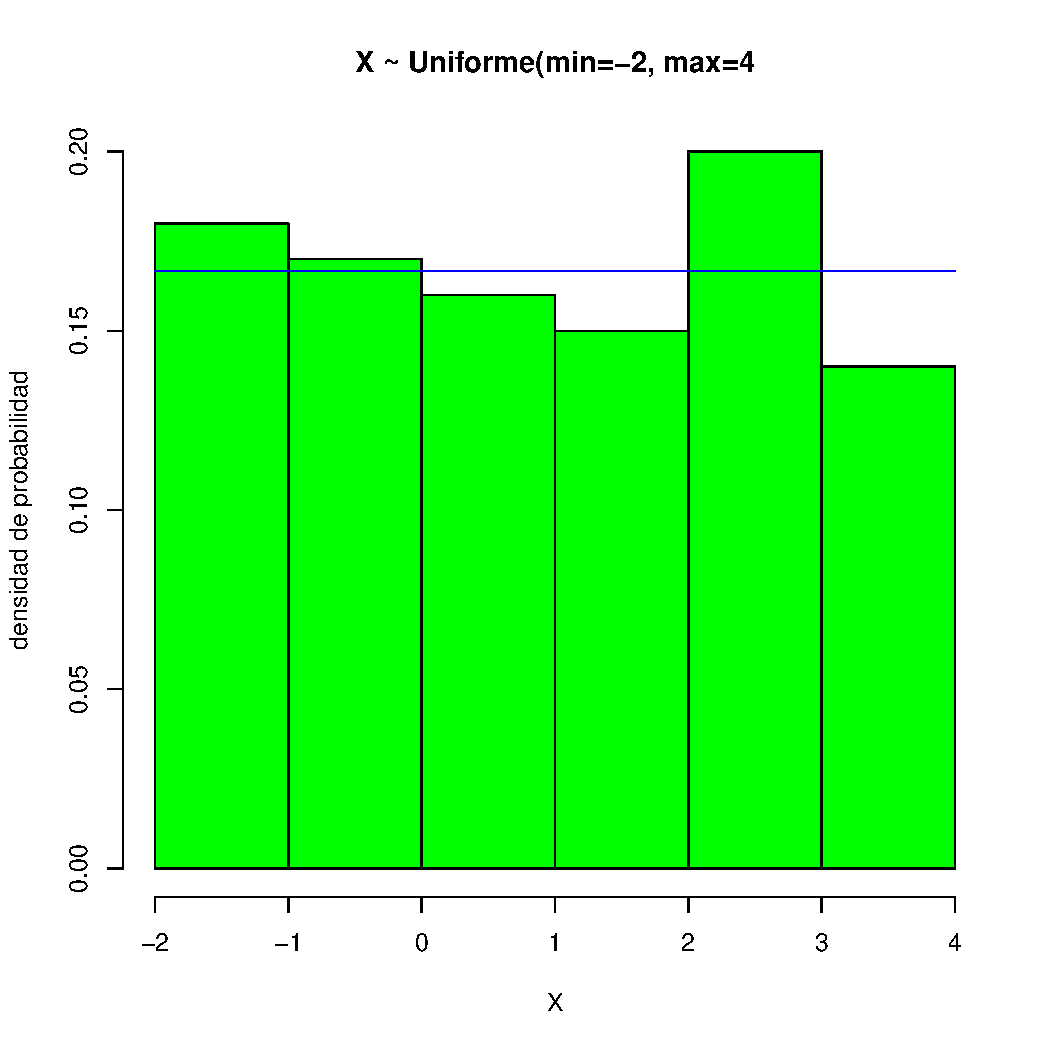
\includegraphics[width=\maxwidth]{figure/unnamed-chunk-15-1} 

\end{knitrout}

\begin{itemize}
  \item \textbf{Ejemplo 2:}
\end{itemize}
Supongamos que tenemos una muestra de tama?o n=200 perteneciente a una poblaci\'on normal N(10,2) con media igual a 10 y con una desviaci\'on estandar igual a 2:
\begin{knitrout}
\definecolor{shadecolor}{rgb}{0.969, 0.969, 0.969}\color{fgcolor}\begin{kframe}
\begin{alltt}
\hlcom{# genera los valores aleatorios de la distribuci\textbackslash{}'on }
\hlstd{x.norm} \hlkwb{<-} \hlkwd{rnorm}\hlstd{(}\hlkwc{n}\hlstd{=}\hlnum{200}\hlstd{,}\hlkwc{mean}\hlstd{=}\hlnum{10}\hlstd{,} \hlkwc{sd}\hlstd{=}\hlnum{2}\hlstd{)}

\hlcom{# Podemos obtener un histograma usando la funci\textbackslash{}'on hist() }
\hlkwd{hist}\hlstd{(x.norm,} \hlkwc{breaks} \hlstd{=} \hlstr{"Sturges"}\hlstd{,} \hlkwc{freq} \hlstd{=} \hlnum{TRUE}\hlstd{,} \hlkwc{probability} \hlstd{=} \hlnum{FALSE}\hlstd{,}
     \hlkwc{include.lowest} \hlstd{=} \hlnum{TRUE}\hlstd{,} \hlkwc{right} \hlstd{=} \hlnum{TRUE}\hlstd{,} \hlkwc{density} \hlstd{=} \hlkwa{NULL}\hlstd{,}
\hlkwc{angle} \hlstd{=} \hlnum{45}\hlstd{,} \hlkwc{col} \hlstd{=} \hlstr{"steelblue1"}\hlstd{,} \hlkwc{border} \hlstd{=} \hlkwa{NULL}\hlstd{,}
\hlkwc{main} \hlstd{=} \hlstr{"Histograma de datos observados"}\hlstd{,} \hlkwc{axes} \hlstd{=} \hlnum{TRUE}\hlstd{,}
\hlkwc{plot} \hlstd{=} \hlnum{TRUE}\hlstd{,} \hlkwc{labels} \hlstd{=} \hlnum{FALSE}\hlstd{)}
\end{alltt}
\end{kframe}
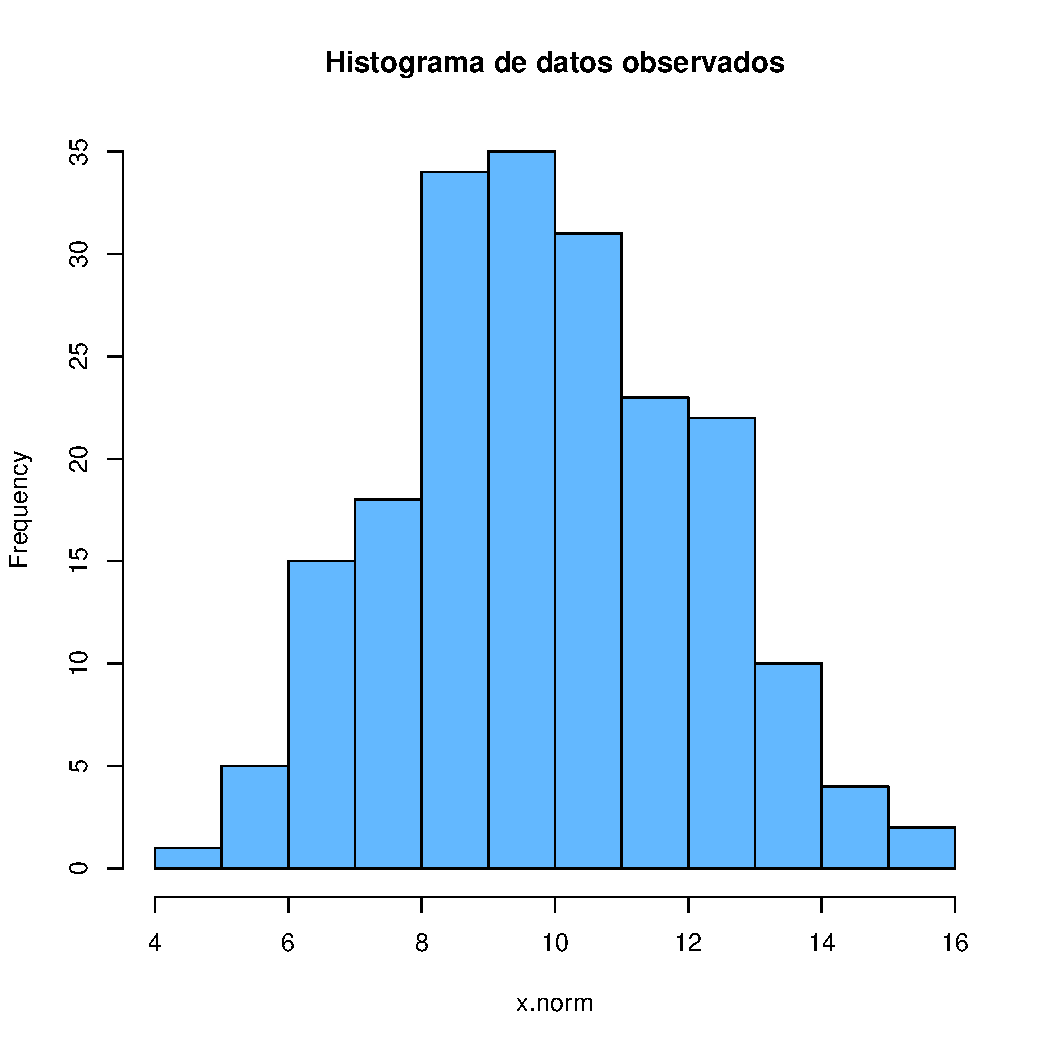
\includegraphics[width=\maxwidth]{figure/unnamed-chunk-16-1} 
\begin{kframe}\begin{alltt}
\hlcom{# Podemos estimar la densidad de frecuencia usando la funci\textbackslash{}'on }
\hlcom{# density() y plot() para dibujar su "gr\textbackslash{}'afica"}
\hlkwd{plot}\hlstd{(}\hlkwd{density}\hlstd{(x.norm),} \hlkwc{main}\hlstd{=}\hlstr{"Densidad estimada de los datos"}\hlstd{)}
\end{alltt}
\end{kframe}
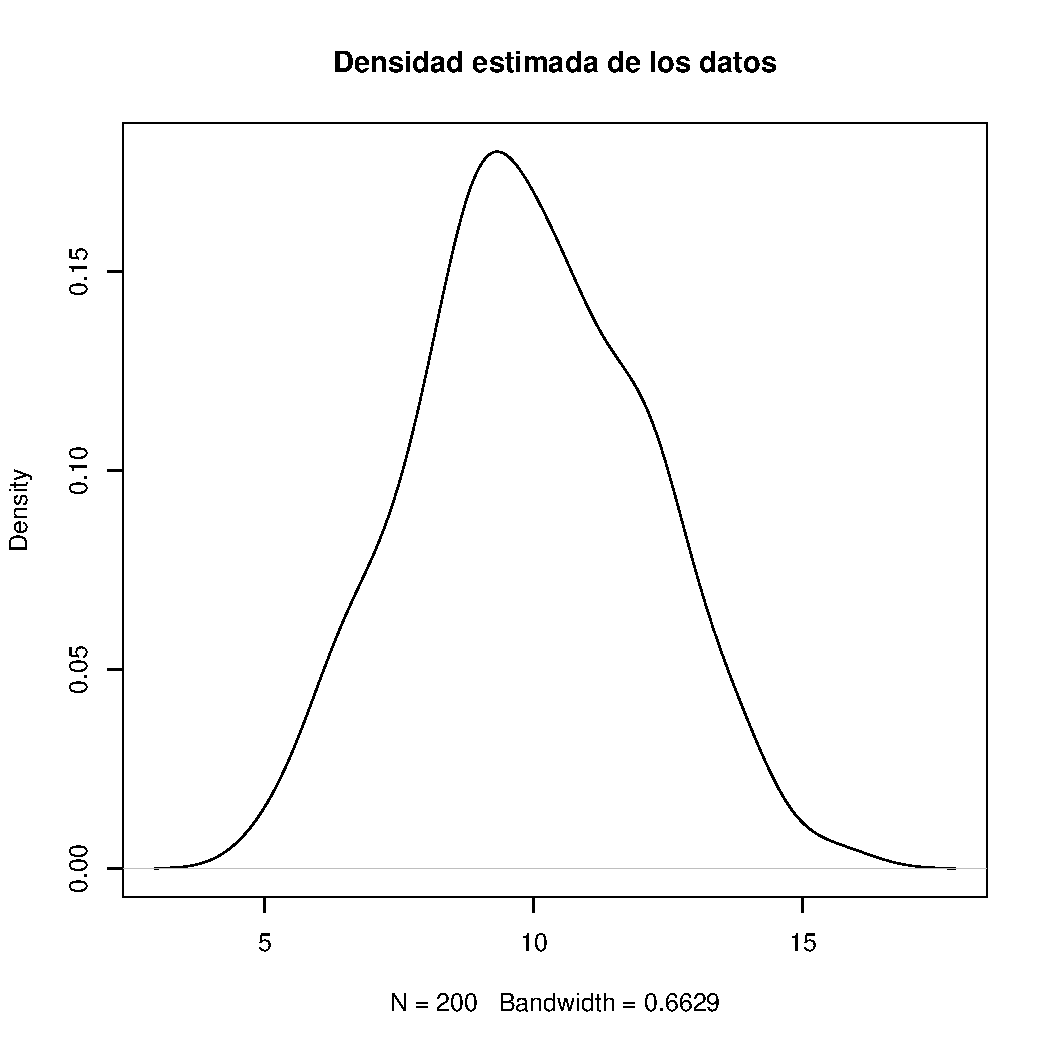
\includegraphics[width=\maxwidth]{figure/unnamed-chunk-16-2} 
\begin{kframe}\begin{alltt}
\hlcom{# R permite calcular la funci\textbackslash{}'on de distribuci\textbackslash{}'on acumulada te\textbackslash{}'erica con ecdf() }
\hlkwd{plot}\hlstd{(}\hlkwd{ecdf}\hlstd{(x.norm),}\hlkwc{main}\hlstd{=}\hlstr{"Funcion de distribucion acumulada teorica"}\hlstd{)}
\end{alltt}
\end{kframe}
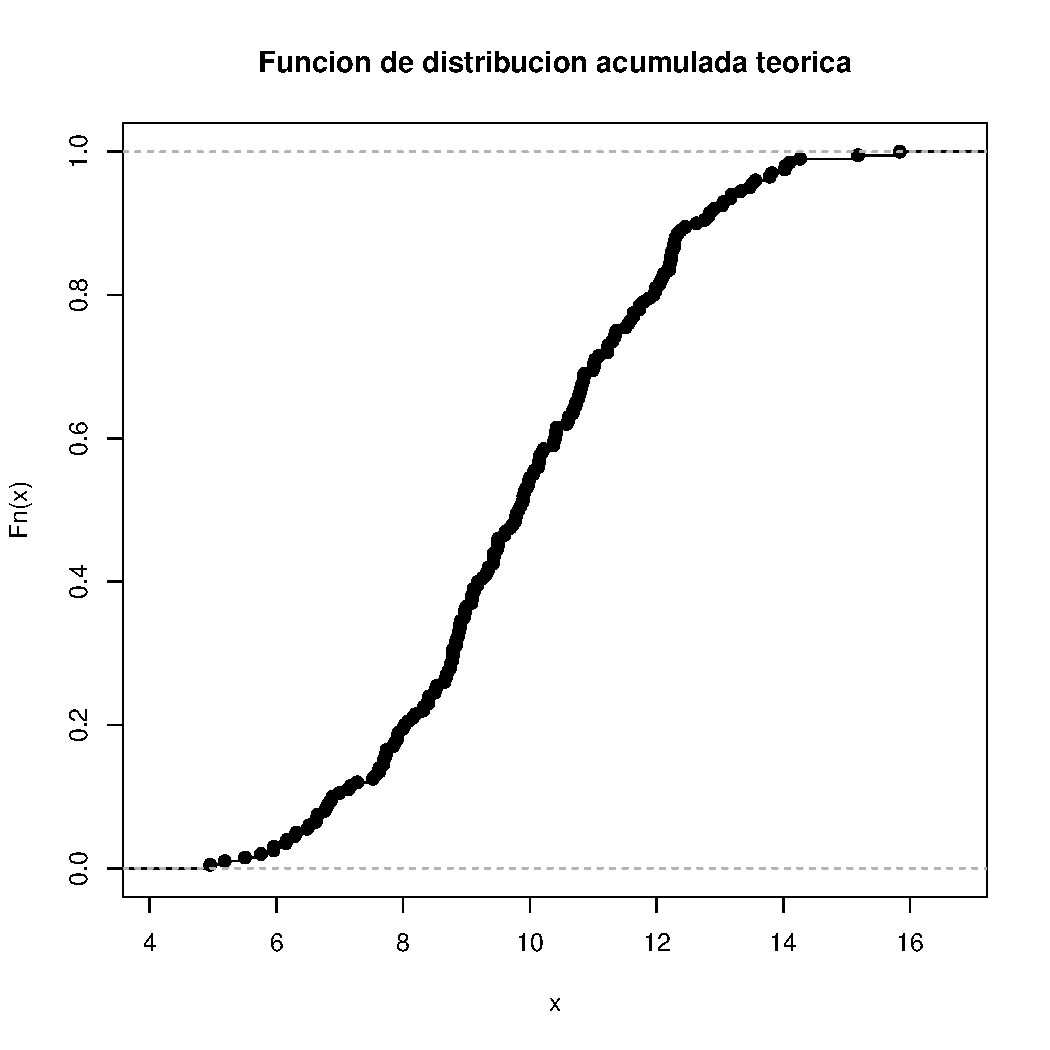
\includegraphics[width=\maxwidth]{figure/unnamed-chunk-16-3} 

\end{knitrout}

\begin{itemize}
  \item \textbf{Ejemplo 3:}
\end{itemize}
Generar 100 n\'umeros aleatorios de una distribuci\'on Normal con media 4.5 y desviaci\'on est\'andar 0.75.
\begin{knitrout}
\definecolor{shadecolor}{rgb}{0.969, 0.969, 0.969}\color{fgcolor}\begin{kframe}
\begin{alltt}
\hlcom{# Definir los par\textbackslash{}'ametros apropiados }
\hlstd{media} \hlkwb{<-} \hlnum{4.5}\hlstd{; desviacion} \hlkwb{<-} \hlnum{0.75}

\hlcom{# generar 100 n\textbackslash{}'umeros aleatorios de la distribuci\textbackslash{}'on }
\hlstd{x} \hlkwb{=} \hlkwd{rnorm}\hlstd{(}\hlnum{100}\hlstd{, media, desviacion); x}
\end{alltt}
\begin{verbatim}
##   [1] 5.114109 2.807644 4.829150 5.171246 3.324950 4.806662 4.467318
##   [8] 3.822467 4.808454 5.475646 4.288946 6.035396 2.796695 4.633310
##  [15] 4.344524 5.138528 3.687893 4.497320 5.129663 3.855692 5.467961
##  [22] 5.433751 4.242510 3.398178 3.172333 4.440449 4.681502 4.417731
##  [29] 3.910563 5.505933 4.454395 4.282156 3.772408 3.953513 3.592070
##  [36] 4.103023 3.303338 4.960042 4.145200 4.781578 4.423927 5.332887
##  [43] 4.188500 3.830366 5.305644 4.392712 4.124634 3.233090 4.493575
##  [50] 4.508792 4.262792 3.862822 5.890693 3.961443 3.701477 2.362809
##  [57] 4.433050 4.660429 2.928642 5.798794 3.842752 4.021842 4.438447
##  [64] 4.291631 2.820015 4.939433 4.441936 4.702720 4.858302 4.623014
##  [71] 3.903635 3.405556 4.337589 4.901855 4.112485 4.775759 4.720916
##  [78] 3.938021 4.889683 3.802883 2.264697 4.477672 3.510906 3.964042
##  [85] 4.309669 4.369897 3.784581 5.534855 4.089908 5.285568 4.188865
##  [92] 4.044965 3.245994 4.484572 4.532582 5.871118 3.531160 5.417253
##  [99] 3.920462 4.870577
\end{verbatim}
\begin{alltt}
\hlcom{# Histograma para la nuestra aleatoria de tama\textbackslash{}~no 100 }
\hlkwd{hist}\hlstd{(x,}\hlkwc{main}\hlstd{=}\hlkwd{expression}\hlstd{(}\hlkwd{paste}\hlstd{(}\hlstr{"X ~ N("}\hlstd{, mu,} \hlstr{" = 4.5, "}\hlstd{, sigma,} \hlstr{" = 0.75)"}\hlstd{)),}
\hlkwc{xlab}\hlstd{=}\hlstr{"X"}\hlstd{,} \hlkwc{ylab}\hlstd{=}\hlstr{"densidad de probabilidad"}\hlstd{,} \hlkwc{probability}\hlstd{=}\hlnum{TRUE}\hlstd{,} \hlkwc{col}\hlstd{=}\hlkwd{gray}\hlstd{(}\hlnum{0.9}\hlstd{))}

\hlcom{# Graficar la funci\textbackslash{}'on de densidad te\textbackslash{}'orica, usando la funci\textbackslash{}'on curve() }
\hlkwd{curve}\hlstd{(}\hlkwd{dnorm}\hlstd{(x, media, desviacion),} \hlkwc{col}\hlstd{=}\hlstr{"red"}\hlstd{,} \hlkwc{lwd}\hlstd{=}\hlnum{2}\hlstd{,} \hlkwc{add}\hlstd{=}\hlnum{TRUE}\hlstd{)}
\end{alltt}
\end{kframe}
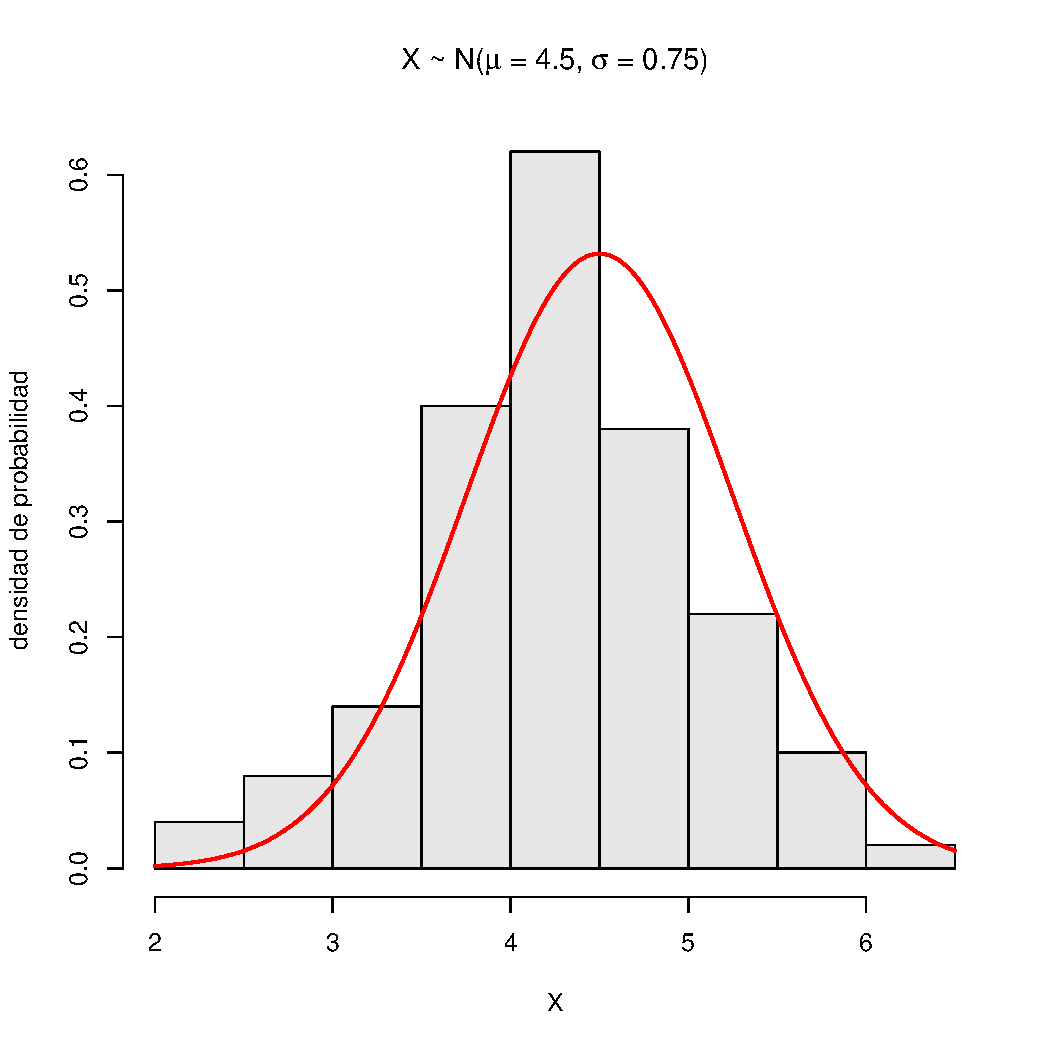
\includegraphics[width=\maxwidth]{figure/unnamed-chunk-17-1} 

\end{knitrout}

\begin{itemize}
  \item \textbf{Ejemplo 4:}
\end{itemize}
Generar n\'umeros aleatorios de una distribuci\'on exponencial. Por ejemplo, si la vida media de un bulbo de luz es 2500 horas, uno puede pensar que el tiempo de vida es aleatorio con una distribuci\'on exponencial que tiene media 2500. El \'unico par\'ametro es la raz\'on = 1/media.
\begin{knitrout}
\definecolor{shadecolor}{rgb}{0.969, 0.969, 0.969}\color{fgcolor}\begin{kframe}
\begin{alltt}
\hlcom{# Definir el par?metro apropiado }
\hlstd{media} \hlkwb{<-} \hlnum{2500}\hlstd{; razon} \hlkwb{<-} \hlnum{1}\hlopt{/}\hlstd{media;n}\hlkwb{=}\hlnum{100}

\hlcom{# generar 100 n\textbackslash{}'umeros aleatorios de la distribuci\textbackslash{}'on }
\hlstd{x} \hlkwb{=} \hlkwd{rexp}\hlstd{(n, razon); x}
\end{alltt}
\begin{verbatim}
##   [1]   901.95372   156.02655   314.37034   686.53587  2168.73472
##   [6] 12610.37500  1294.54967  5037.86508   790.48373  1459.89267
##  [11]   544.09025  1792.61143   623.46199  1082.83775  1880.64956
##  [16]  3750.12424   947.67923   171.12897  1378.74409  1827.84653
##  [21]  3514.88976   987.83332  4675.25531   125.15029  2301.93588
##  [26]  4880.12586  4294.12533   453.92363   615.54986  4105.06456
##  [31]  8990.30009  2009.22687  1283.46889  1985.75671   846.18787
##  [36]  7525.72266  1879.99209  1568.82495  4406.31317  3615.10507
##  [41]   710.79347  2806.97688  1207.28220   402.94989   510.31647
##  [46]    13.69918  3920.24207  3300.66863   841.73483  1199.69926
##  [51]   128.54102  1398.71862  2539.67809  1096.25286   595.05019
##  [56]  2913.33995  1608.20961  1941.50742   631.51822  5902.51131
##  [61]  6806.67411  2136.95224  4760.77787   967.67014  3757.59341
##  [66]   378.41600  4074.94374  4715.03219  1862.15400   890.88257
##  [71]    36.01121   732.54459   171.37922  7761.43933  2318.60703
##  [76]  1422.16634  1026.25208   847.59358  2294.66934  1247.00699
##  [81]  2777.53470  2710.36026  5869.33780  1807.00381  2265.43562
##  [86]  6032.54183  2236.81901   247.31747  2863.80081   417.88469
##  [91]  6051.81204  6161.00521   112.80848   835.06331   350.41069
##  [96]  2427.17627   466.93276  7923.93098  3617.30096  7741.74010
\end{verbatim}
\begin{alltt}
\hlcom{# Histograma para la nuestra aleatoria de tama\textbackslash{}~no 100 }
\hlkwd{hist}\hlstd{(x,} \hlkwc{main}\hlstd{=}\hlstr{"X ~ Exponencial( media = 2500 )"}\hlstd{,} \hlkwc{xlab}\hlstd{=}\hlstr{"X"}\hlstd{,}
     \hlkwc{ylab}\hlstd{=}\hlstr{"densidad de probabilidad"}\hlstd{,} \hlkwc{probability}\hlstd{=}\hlnum{TRUE}\hlstd{,} \hlkwc{col}\hlstd{=}\hlstr{"green"}\hlstd{)}

\hlcom{# Graficar la funci?n de densidad, usando la funci?n curve() }
\hlkwd{curve}\hlstd{(}\hlkwd{dexp}\hlstd{(x, razon),} \hlkwc{col}\hlstd{=}\hlstr{"blue"}\hlstd{,} \hlkwc{lwd}\hlstd{=}\hlnum{2}\hlstd{,} \hlkwc{add}\hlstd{=}\hlnum{TRUE}\hlstd{)}
\end{alltt}
\end{kframe}
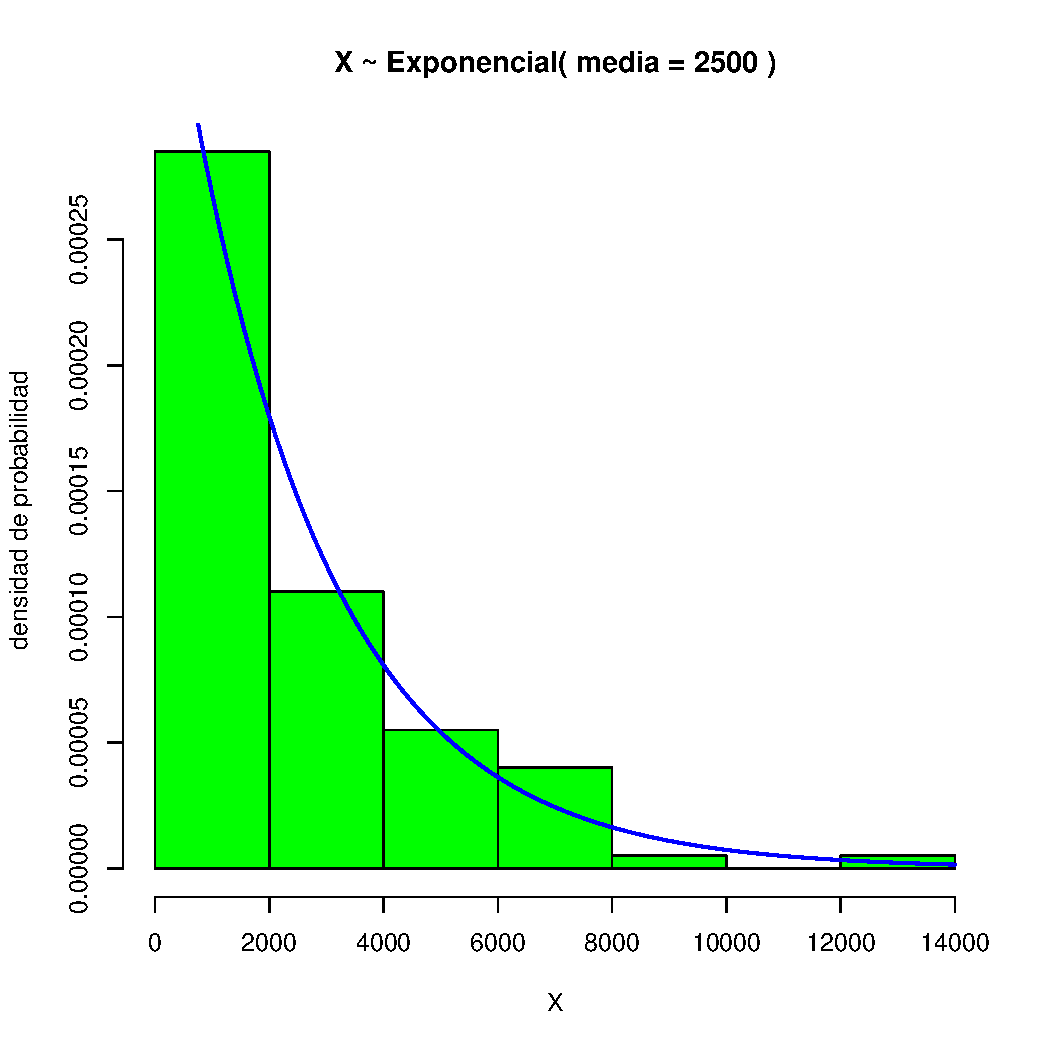
\includegraphics[width=\maxwidth]{figure/unnamed-chunk-18-1} 

\end{knitrout}

\newpage


\section{FUNCIONES DE DISTRIBUCI\'ON Y SU INVERSA (LOS CUANTILES).}


En R, las funciones a las que se les antepone una "p" permiten contestar cu?l es la probabilidad de que una variable aleatoria X sea menor o igual que x, esto es F(x)=P[X$<$=x]. Las funciones a las que se les antepone una "q" son lo inverso de esto, ellas permiten conocer qu\'e valor de una variable aleatoria X corresponde a una probabilidad p dada. Esto es el cuantil Xq o punto en el que los datos son partidos, P[X$<$=x_q]=p.\\

\begin{itemize}
  \item \textbf{Ejemplo 1:}
\end{itemize}
Para una Variable aleatoria X con distribuci\'on normal de media 1 y desviaci\'on 
est\'andar 1, cu\'al es la probabilidad de que sea menor que 0.7?
\begin{knitrout}
\definecolor{shadecolor}{rgb}{0.969, 0.969, 0.969}\color{fgcolor}\begin{kframe}
\begin{alltt}
\hlstd{x} \hlkwb{<-} \hlnum{0.7}
\hlstd{p} \hlkwb{<-} \hlkwd{pnorm}\hlstd{(x,} \hlkwc{mean}\hlstd{=}\hlnum{1}\hlstd{,} \hlkwc{sd}\hlstd{=}\hlnum{1}\hlstd{,} \hlkwc{lower.tail} \hlstd{=} \hlnum{TRUE}\hlstd{); p}
\end{alltt}
\begin{verbatim}
## [1] 0.3820886
\end{verbatim}
\end{kframe}
\end{knitrout}
\textbf{Observaci\'on:} lower.tail=TRUE es el valor por defecto, para indicar las probabilidades son P[X$<$=x], en otro caso ser\'a P[X$>$x].

\begin{itemize}
  \item \textbf{Ejemplo 2:}
\end{itemize}
Para una variable aleatoria con distribuci\'on normal est\'andar, encontrar 
P[Z$<$=0.7] y P[Z$>$0.7]. 
\begin{knitrout}
\definecolor{shadecolor}{rgb}{0.969, 0.969, 0.969}\color{fgcolor}\begin{kframe}
\begin{alltt}
\hlstd{z} \hlkwb{<-} \hlnum{0.7}
\hlstd{p1} \hlkwb{<-} \hlkwd{pnorm}\hlstd{(z,} \hlkwc{mean}\hlstd{=}\hlnum{0}\hlstd{,} \hlkwc{sd}\hlstd{=}\hlnum{1}\hlstd{); p1}
\end{alltt}
\begin{verbatim}
## [1] 0.7580363
\end{verbatim}
\begin{alltt}
\hlstd{p2} \hlkwb{<-} \hlkwd{pnorm}\hlstd{(z,} \hlkwc{mean}\hlstd{=}\hlnum{0}\hlstd{,} \hlkwc{sd}\hlstd{=}\hlnum{1}\hlstd{,} \hlkwc{lower.tail}\hlstd{=}\hlnum{FALSE}\hlstd{); p2}
\end{alltt}
\begin{verbatim}
## [1] 0.2419637
\end{verbatim}
\end{kframe}
\end{knitrout}
\textbf{Observaci\'on:} ya que P[Z$>$0.7]=1-[Z$<$=0.7], obtenemos el mismo resultado con
\begin{knitrout}
\definecolor{shadecolor}{rgb}{0.969, 0.969, 0.969}\color{fgcolor}\begin{kframe}
\begin{alltt}
\hlstd{p3} \hlkwb{<-} \hlnum{1}\hlopt{-}\hlkwd{pnorm}\hlstd{(z,} \hlkwc{mean}\hlstd{=}\hlnum{0}\hlstd{,} \hlkwc{sd}\hlstd{=}\hlnum{1}\hlstd{);p3}
\end{alltt}
\begin{verbatim}
## [1] 0.2419637
\end{verbatim}
\end{kframe}
\end{knitrout}

\begin{itemize}
  \item \textbf{Ejemplo 3:}
\end{itemize}
Qu\'e valor de una variable aleatoria con distribuci\'on normal est\'andar, tiene 75\% 
del ?rea a la izquierda?. 
\begin{knitrout}
\definecolor{shadecolor}{rgb}{0.969, 0.969, 0.969}\color{fgcolor}\begin{kframe}
\begin{alltt}
\hlstd{p} \hlkwb{<-} \hlnum{0.75}
\hlstd{z} \hlkwb{<-} \hlkwd{qnorm}\hlstd{(p,} \hlkwc{mean}\hlstd{=}\hlnum{0}\hlstd{,} \hlkwc{sd}\hlstd{=}\hlnum{1}\hlstd{,} \hlkwc{lower.tail} \hlstd{=} \hlnum{TRUE}\hlstd{); z}
\end{alltt}
\begin{verbatim}
## [1] 0.6744898
\end{verbatim}
\end{kframe}
\end{knitrout}
\textbf{Observaci\'on:} note que el valor de z que resuelve P[Z$<$=z]=0.75 es el tercer cuartil (Q3), esto es z=0.6744898.

\begin{itemize}
  \item \textbf{Ejemplo 4:}
\end{itemize}
Cu\'al es la probabilidad a la derecha de 18.55 para una Variable aleatoria X con 
distribuci\'on Chi-cuadrado de 12 grados de libertad?
\begin{knitrout}
\definecolor{shadecolor}{rgb}{0.969, 0.969, 0.969}\color{fgcolor}\begin{kframe}
\begin{alltt}
\hlstd{x} \hlkwb{<-} \hlnum{18.55}\hlstd{; gl} \hlkwb{<-} \hlnum{12}
\hlstd{p} \hlkwb{<-} \hlkwd{pchisq}\hlstd{(x, gl,} \hlkwc{lower.tail} \hlstd{=} \hlnum{FALSE}\hlstd{); p}
\end{alltt}
\begin{verbatim}
## [1] 0.09998251
\end{verbatim}
\end{kframe}
\end{knitrout}

\end{document}
